%----------------------------------------------------------------------------------------
%	PACKAGES AND THEMES
%----------------------------------------------------------------------------------------
\documentclass[aspectratio=169,xcolor=dvipsnames]{beamer}
%\usetheme{Simple}

\usepackage{hyperref}
\usepackage{graphicx} % Allows including images
\usepackage{booktabs} % Allows the use of \toprule, \midrule and \bottomrule in tables

\usepackage[ngerman]{babel}
\usepackage{caption}
\usepackage{xcolor}

% Seitennummer unten rechts anzeigen
\setbeamertemplate{footline}[text line]{
  \hfill\insertframenumber{} / \inserttotalframenumber\hspace{0.5em}\vspace{0.3em}
}

\setbeamertemplate{navigation symbols}{}

\captionsetup[figure]{labelformat=simple, labelsep=colon, name=Abb.}

%----------------------------------------------------------------------------------------
%	TITLE PAGE
%----------------------------------------------------------------------------------------

% The title
\title[short title]{Armutsfaktoren im London des 19. Jahrhunders }
%\subtitle{Part 2}

\author[Xuan-Loc Tran] {Leonie Abels, Amirreza Ahmadi Darani, Aziz Klebleyev, Bjarne Möller, Franz Müller, Xuan-Loc Tran}
\institute[NTU] % Your institution may be shorthand to save space
{
    % Your institution for the title page
    Data-Analytics \\
    Prof. Dr. Jill Klünder \\
    FHDW Hannover
    \vskip 3pt
}
\date{\today} % Date, can be changed to a custom date


%----------------------------------------------------------------------------------------
%	PRESENTATION SLIDES
%----------------------------------------------------------------------------------------

\begin{document}

\begin{frame}
    % Print the title page as the first slide
    \titlepage
\end{frame}

\begin{frame}{Gliederung}
    % Throughout your presentation, if you choose to use \section{} and \subsection{} commands, these will automatically be printed on this slide as an overview of your presentation
    \tableofcontents
\end{frame}

%------------------------------------------------
\section{Einführung}
%------------------------------------------------

% was ist eine page
% was ist eine MMU
%%

\begin{frame}{Einführung}
    \begin{itemize}
        \item Wohlstandsforschung aus 19. Jahrhundert
        \item Datenerhebung und Analyse durch Soziologen Charles Booth
        \item Datenerhebung in Schriftsatz
        \item Statistische Tabellen und farbcodierte Armutsdarstellung auf Landkarten
        \item Rein deskriptive Datenerfassung
        \item Wertgewinn des Projekts: Überprüfung alter Datenanalysen mit modernen Methoden
    \end{itemize}
\end{frame}

\section{Fragestellung}
\begin{frame}{Fragestellung}
    \textbf{Welche Faktoren bestimmen die Armut im London des 19. Jahrhunderts?}
\end{frame}


\section{Datenbeschaffung und Aufbereitung}
\begin{frame}{Übertragung bestehender Datensätze} % use case diagram
    \centering
    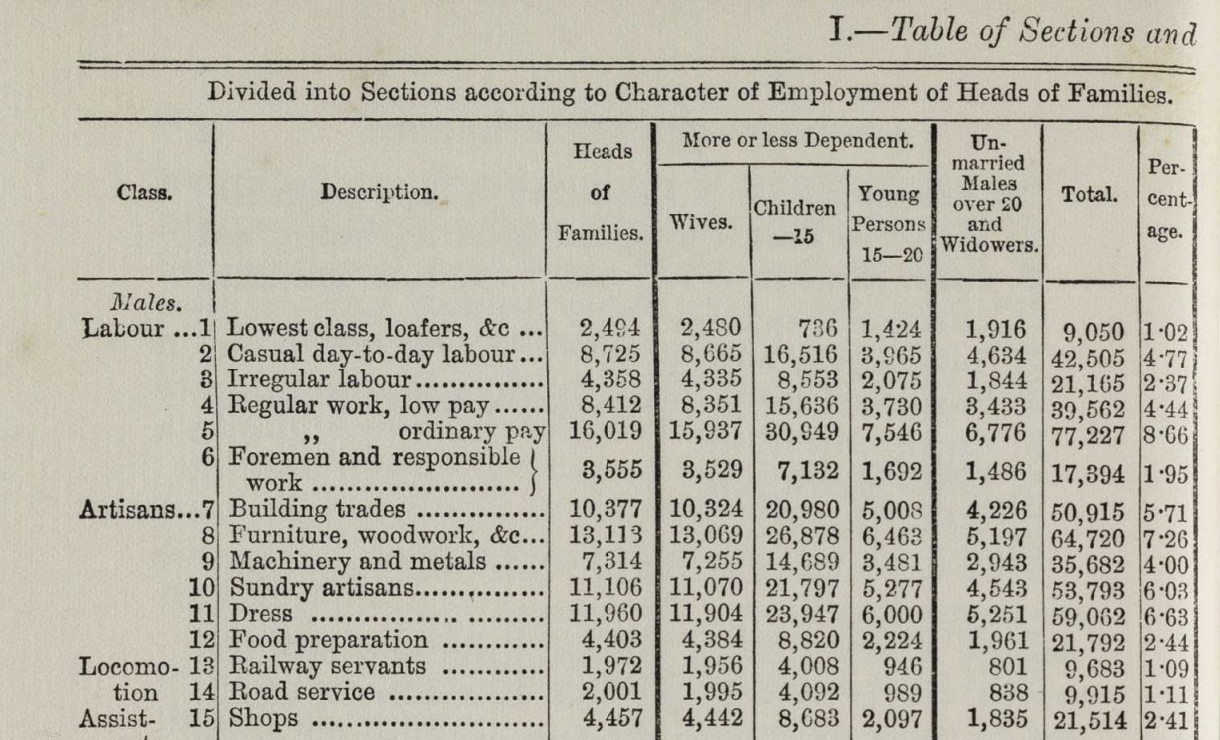
\includegraphics[
    width=\textwidth,
    height=0.8\textheight,
    keepaspectratio
]{abb/booo.png}
\end{frame}


\section{Datenanalyse}
\begin{frame}{Klassifikation sozialer Schichten}
\scriptsize
\centering
\textbf{Charles Booths Klassifikation sozialer Schichten}
\label{tab:booth_classes}

\begin{tabular}{|c|p{4.8cm}|c|p{3.8cm}|}
\hline
\textbf{Class} & \textbf{Description} & \textbf{Category} & \textbf{Category Description} \\
\hline

A & The lowest class of occasional labourers, loafers &
very poor \& semi-criminal &
Lowest Class \\
\hline

B & Casual earnings -- ``very poor'' [semi-criminals] &
very poor \& semi-criminal &
Casual Earnings \\
\hline

C & Intermittent earnings &
poor &
Irregular Earnings \\
\hline

D & Small regular earnings &
poor &
Regular Minimum \\
\hline

E & Regular standard earnings &
comfortable &
Ordinary Standard Earnings \\
\hline

F & Higher class labour &
comfortable &
Highly Paid Work \\
\hline

G & Lower middle class &
well to do &
Lower Middle \\
\hline

H & Upper middle class &
well to do &
Upper Middle \\
\hline

\end{tabular}

\end{frame}
%------------------------------------------------

%------------------------------------------------

%------------------------------------------------

% was ist eine page
% was ist eine MMU
%%

\begin{frame}{Klassenrad aller Daten} % use case diagram
    \centering
    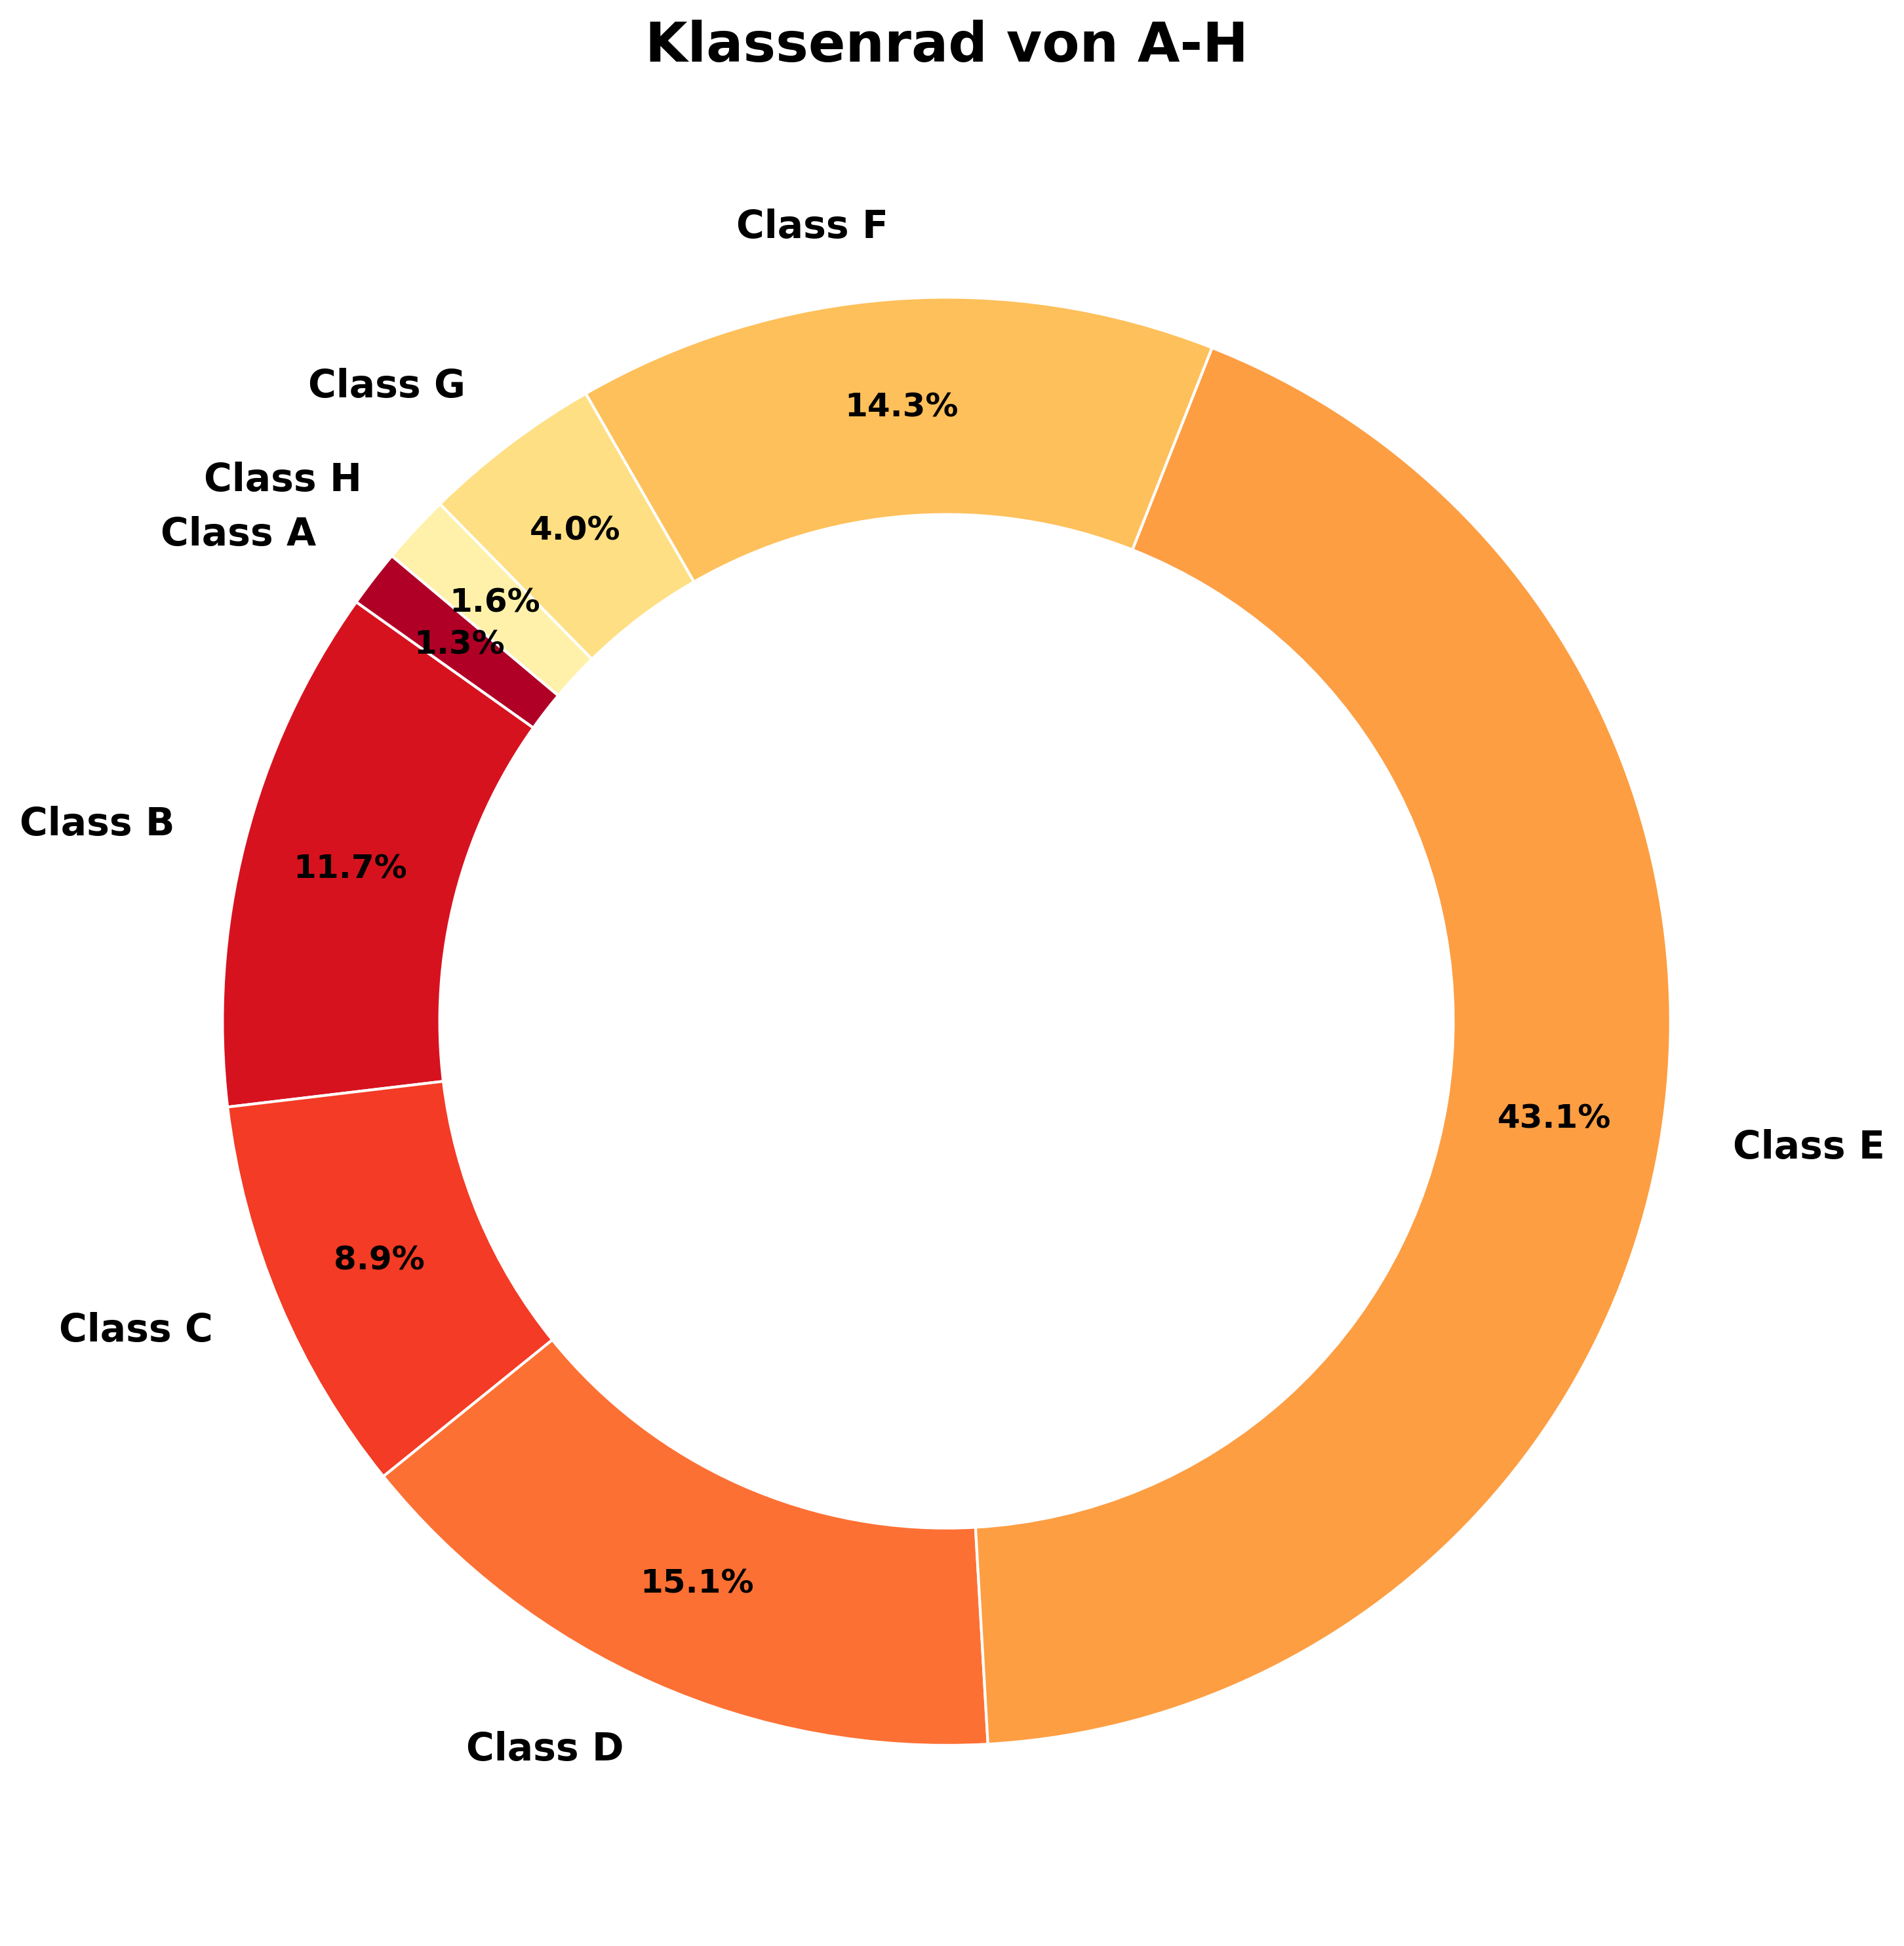
\includegraphics[
    width=\textwidth,
    height=0.8\textheight,
    keepaspectratio
]{abb/poverty_donut.png}
\end{frame}

%----------------------------------------------------------------------------------------




\begin{frame}{Armutsrate nach Boroughs} % use case diagram
    \centering
    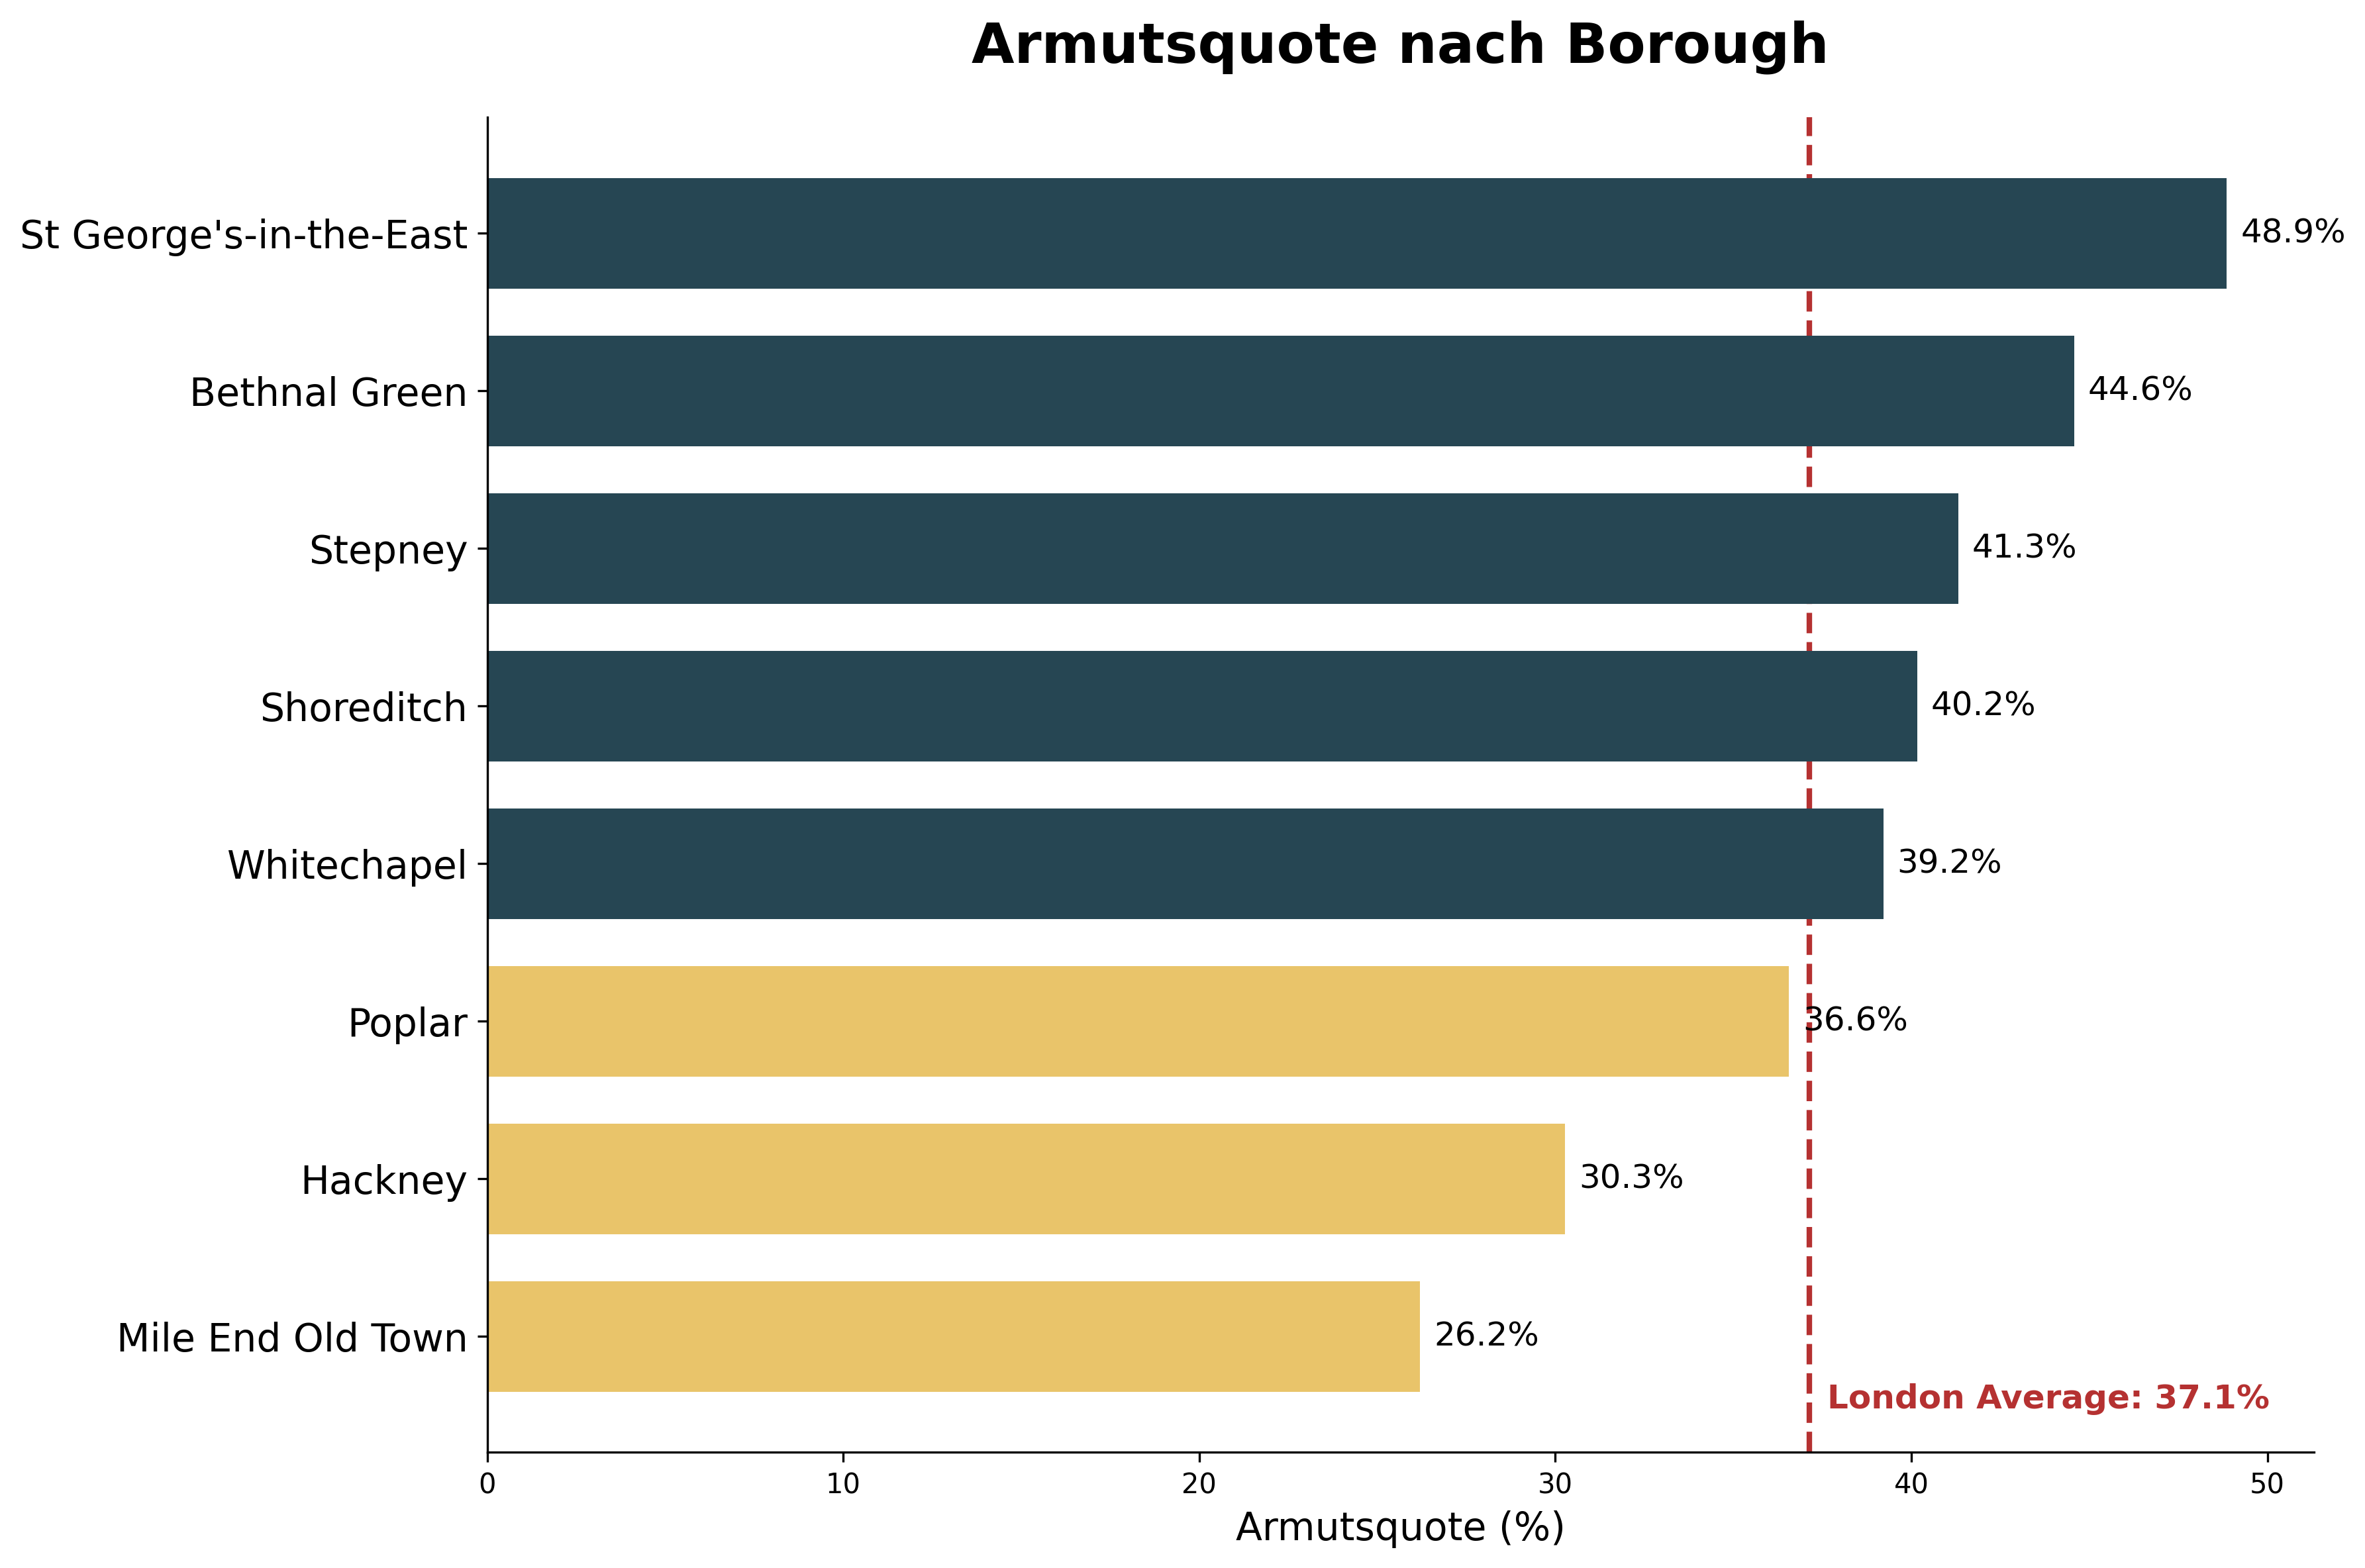
\includegraphics[
    width=\textwidth,
    height=0.8\textheight,
    keepaspectratio
]{abb/city_contrasts_gauge.png}
\end{frame}

\begin{frame}{Joblandschaft und Armutsrisiko} % use case diagram
    \centering
    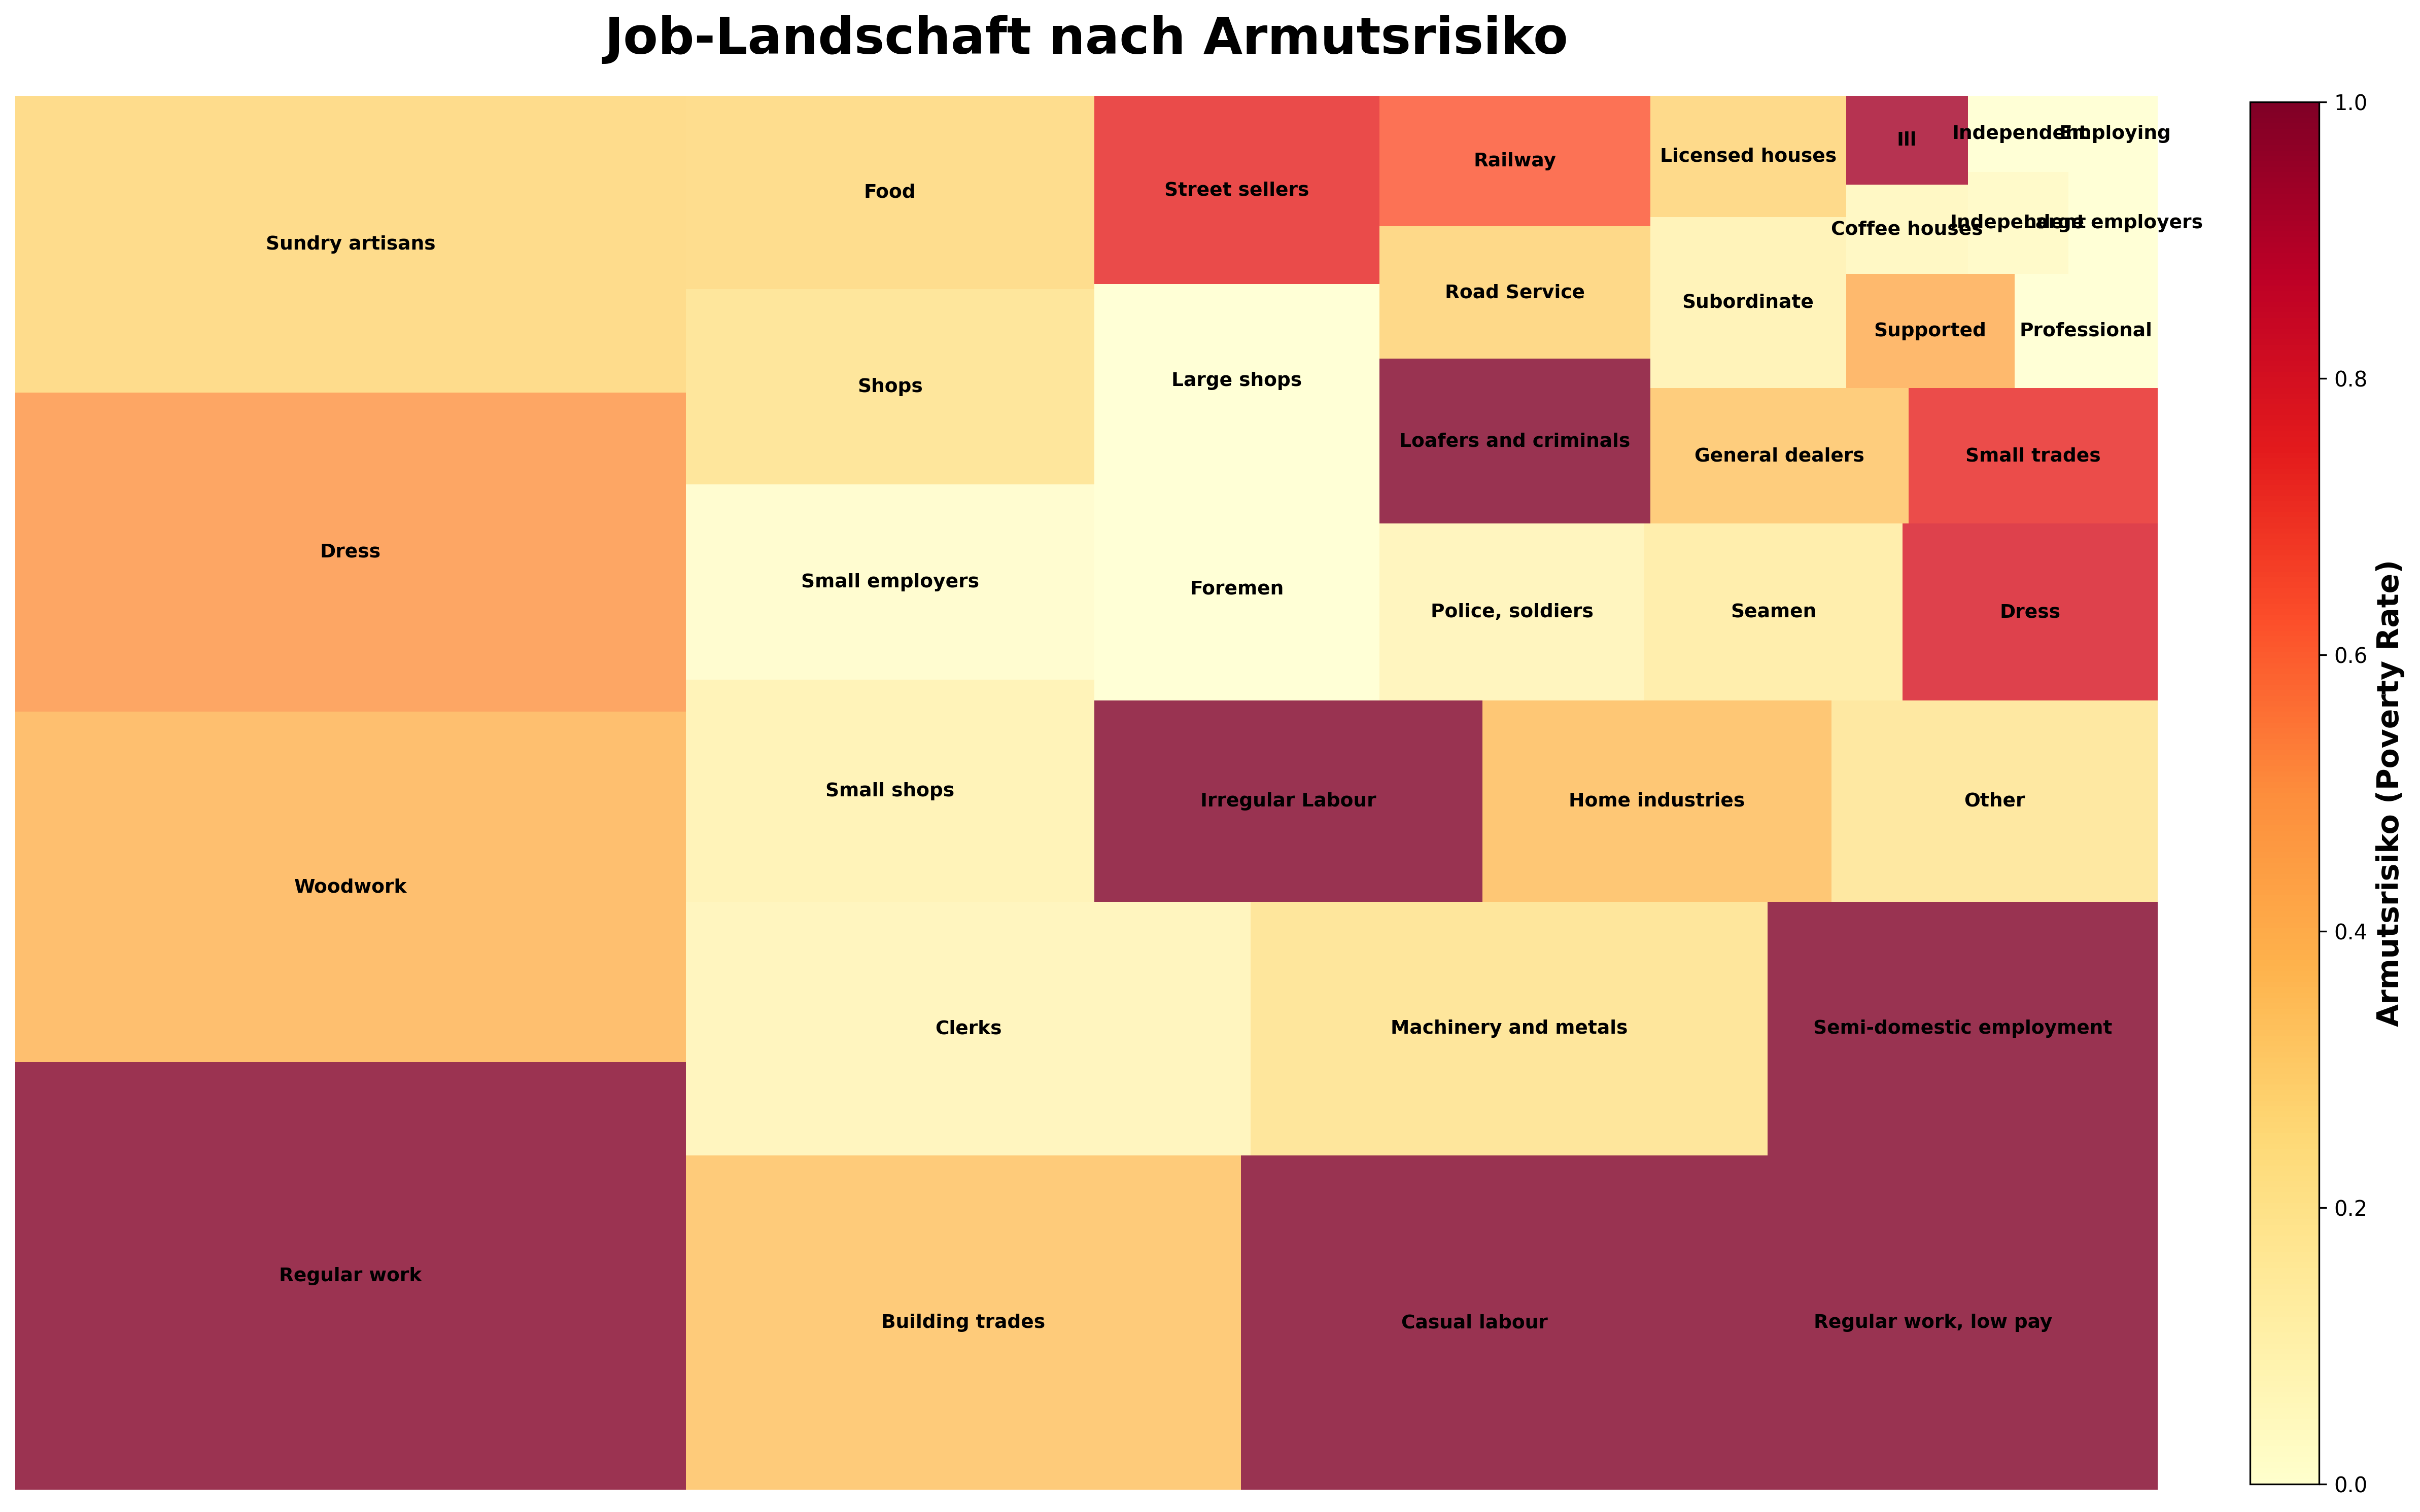
\includegraphics[
    width=\textwidth,
    height=0.8\textheight,
    keepaspectratio
]{abb/job_landscape_treemap.png}
\end{frame}

\begin{frame}{Kinder pro Haushalt und Berufsgruppe} % use case diagram
    \centering
    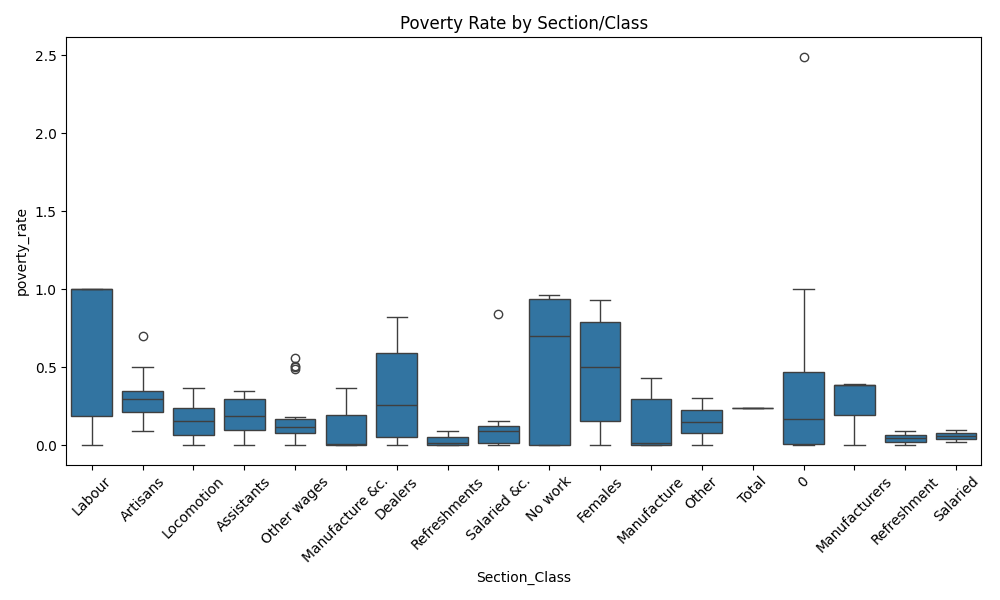
\includegraphics[
    width=\textwidth,
    height=0.8\textheight,
    keepaspectratio
]{abb/boxplot_poverty_rate.png}
\end{frame}

\begin{frame}{Frauen im Armutsdatensatz} % use case diagram
    \centering
    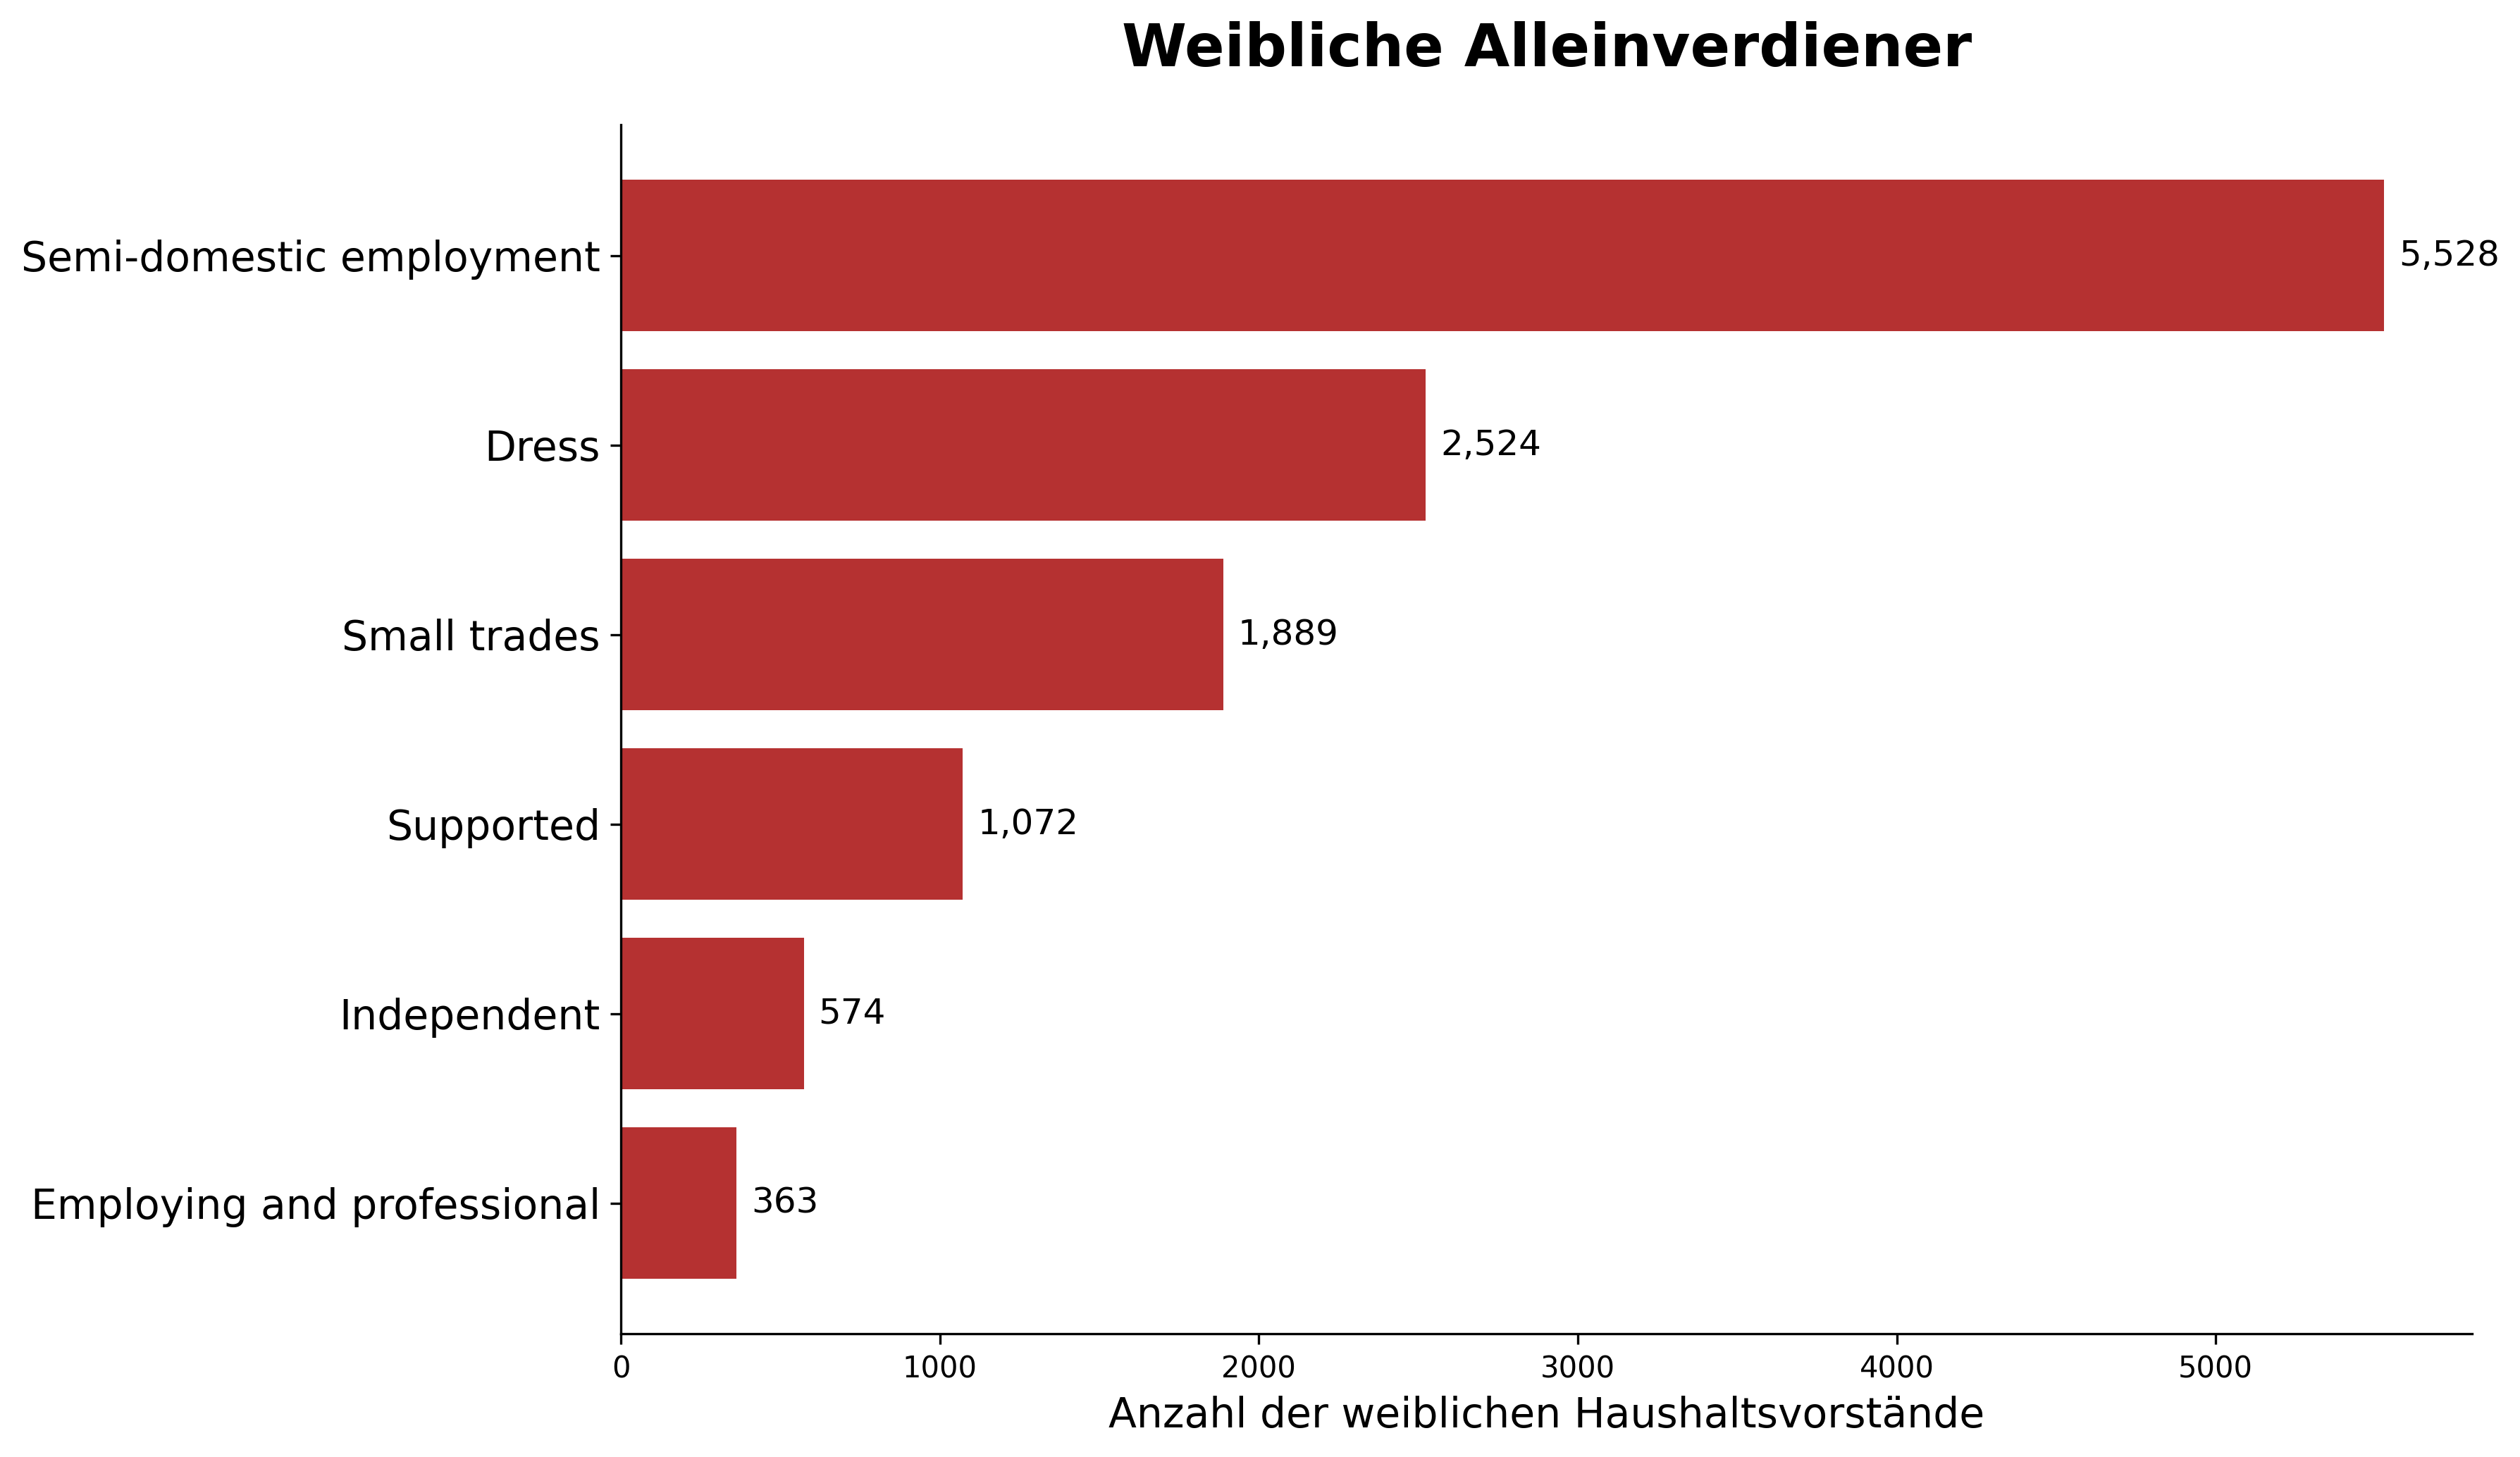
\includegraphics[
    width=\textwidth,
    height=0.8\textheight,
    keepaspectratio
]{abb/invisible_women_bar.png}
\end{frame}

\begin{frame}{Kinder pro Haushalt und Berufsgruppe} % use case diagram
    \centering
    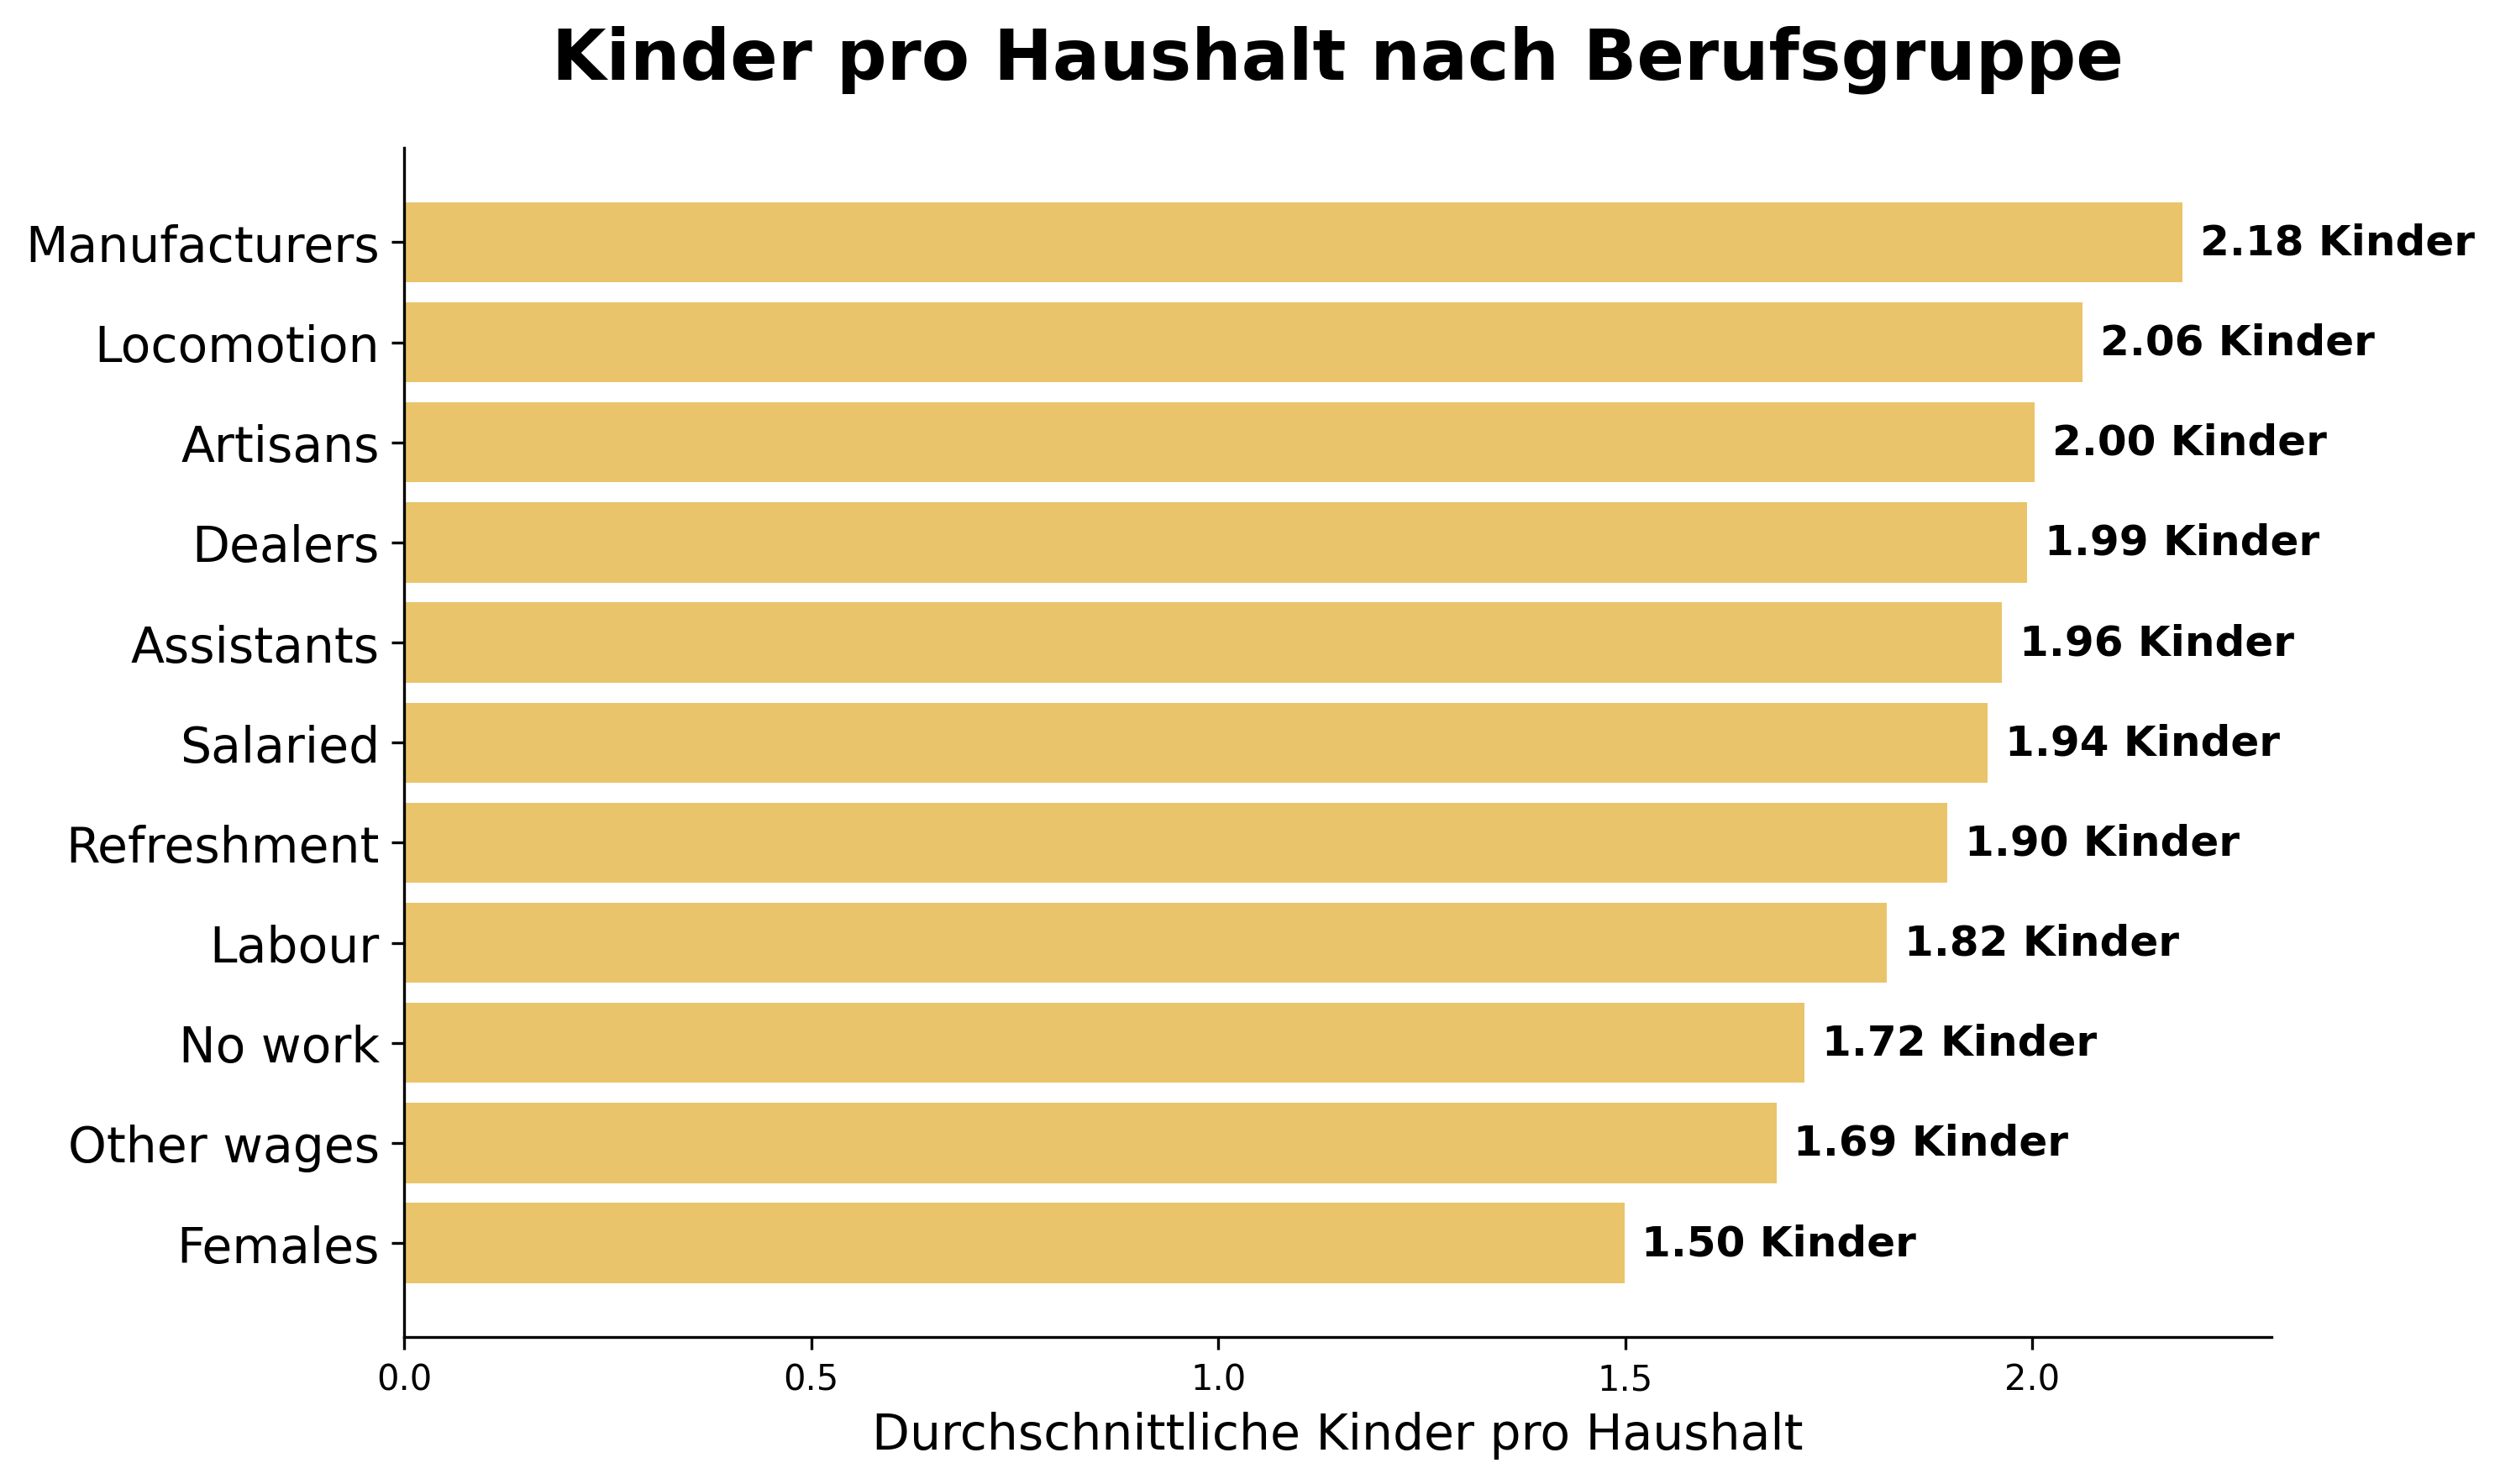
\includegraphics[
    width=\textwidth,
    height=0.8\textheight,
    keepaspectratio
]{abb/living_environments_bar.png}
\end{frame}


\section{Ergebnisse und Ausblick}
%------------------------------------------------

\begin{frame}{Ergebnisse}

    test test
    \begin{itemize}
        \item \textcolor{red}{Labourjobs besonders armutsanfällig:} 
        \begin{itemize}
            \item \textcolor{red}{Tagediebe, Kriminelle}
            \item \textcolor{red}{Gelegenheitsarbeiter bis zu Vollzeitarbeiter}
            \item \textcolor{green}{Schichtleiter und Personalverantwortung}
        \end{itemize}
        \item \textcolor{red}{Weibliche Alleinverdiener besonders armutsanfällig}
        \item \textcolor{green}{Angestellte in Verkauf und Gastgewerbe wenig armutsanfällig}
    \end{itemize}
    %\begin{figure}
    %\includegraphics[width=0.8\linewidth]{abb/pic.jpeg}
    %\caption{Stonehenge}
    %\end{figure}
\end{frame}

\begin{frame}{Ergebnisse}

    test test
    \begin{itemize}
        \item \textcolor{red}{Weibliche Alleinverdiener besonders armutsanfällig}
        \item \textcolor{green}{--> Männliche Alleinverdiener nicht armutsanfällig}
        \item \textcolor{green}{Anzahl der Kinder hat nur geringen Einfluss auf Armut}
    \end{itemize}
    %\begin{figure}
    %\includegraphics[width=0.8\linewidth]{abb/pic.jpeg}
    %\caption{Stonehenge}
    %\end{figure}
\end{frame}

\begin{frame}{Güte und Belastbarkeit des Modells}
    \begin{itemize}
        \item 23,8\% Varianz der Armutsrate abgedeckt
        \item --> Großteil der Varianz ungeklärt
        \item keine Komplettabdeckung durch gegebene Daten
        \item ledigliche Korrelationswerte
    \end{itemize}
\end{frame}

\begin{frame}{Learnings}
    \begin{itemize}
        \item 
        \item 
        \item 
    \end{itemize}
\end{frame}


\begin{frame}{Vielen Dank}
    Vielen Dank
    %\begin{figure}
    %\includegraphics[width=0.8\linewidth]{abb/pic.jpeg}
    %\caption{Stonehenge}
    %\end{figure}
\end{frame}

%----------------------------------------------------------------------------------------




\end{document}
